\newpage
\section{Umsetzung} 
\label{kap:Umsetzung}
\textit{(ygu)} Dieses Kapitel befasst sich mit der technischen Umsetzung des ausgewählten Konzepts aus Kapitel \ref{konzept}. Dabei werden auf alle technischen Details eingegangen, die zur Dokumentation relevant erscheinen. Weitere technische Daten sind aus den entsprechenden Fertigungsunterlagen im Anhang zu entnehmen. Dieses Kapitel ist nach Teilfunktionen gegliedert. 
\subsection{Überblick}
\textit{(ygu)} Der Pflanzroboter bildet eine Einheit, bestehend aus (siehe Legende in Abbildung \ref{fig:uberblick}):
	\begin{figure}[H]
	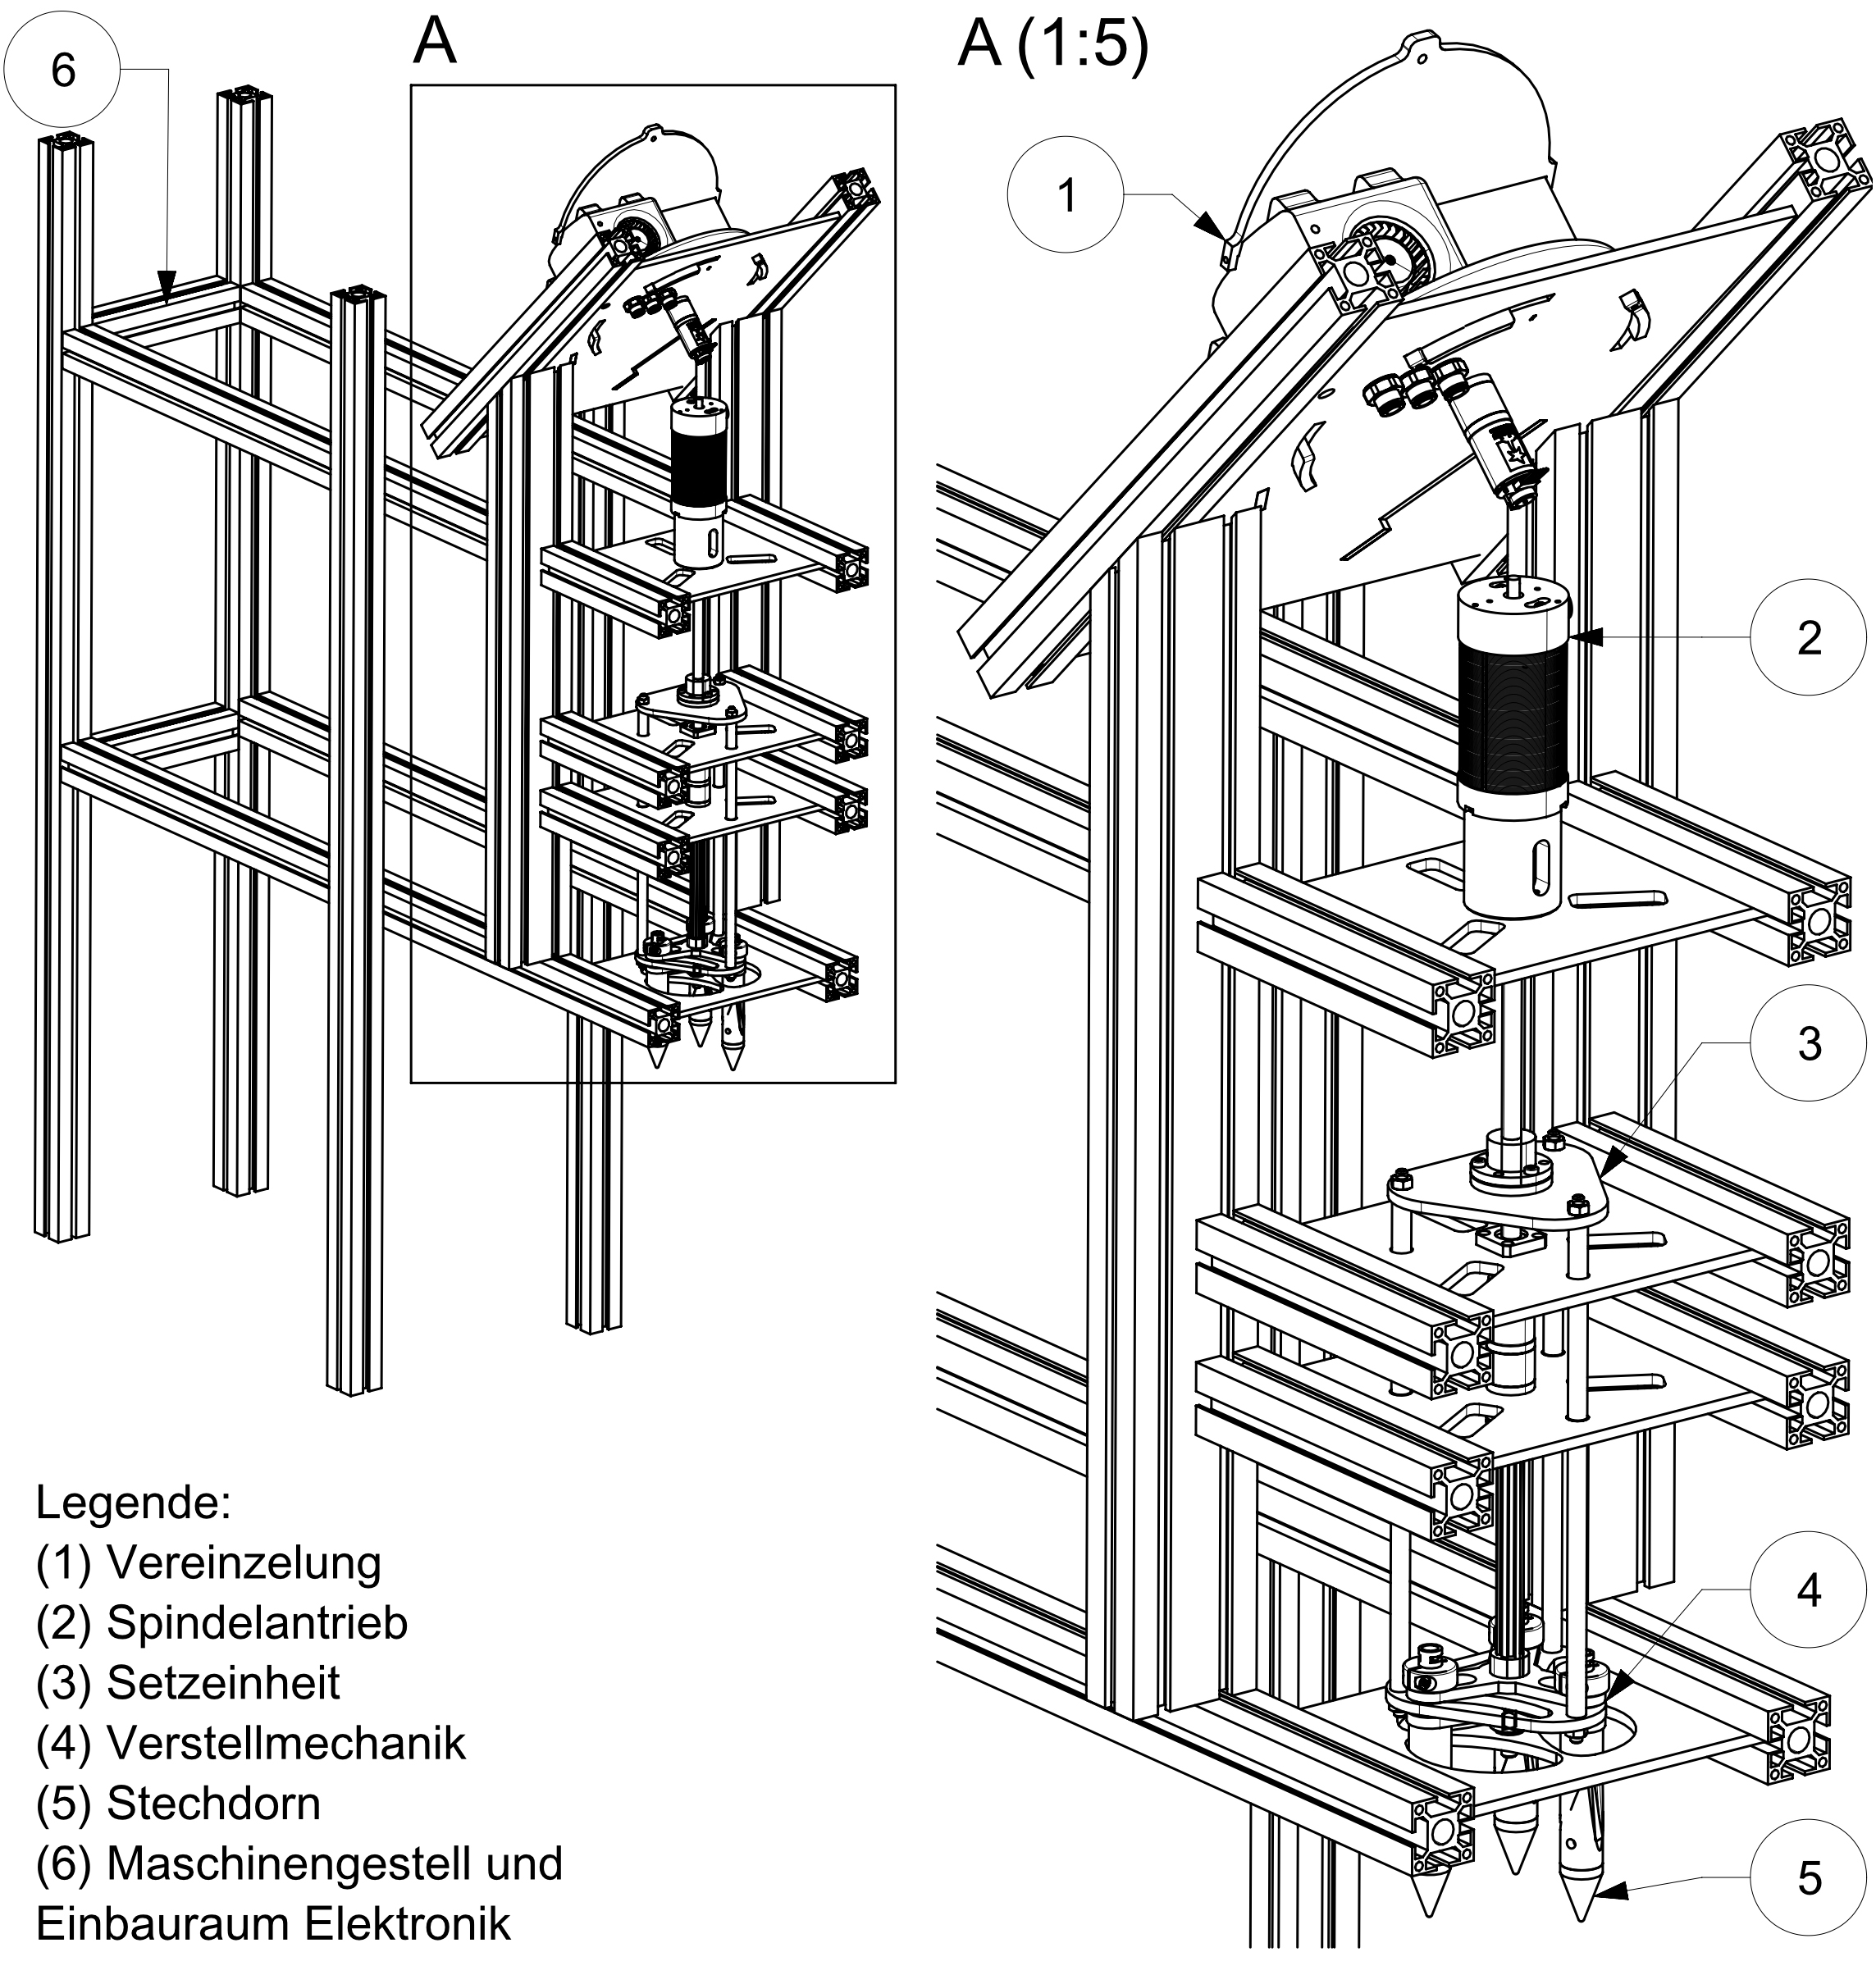
\includegraphics[scale=0.75]{Illustrationen/6-Umsetzung/uberblick.jpg}
	\caption{Perspektivische Ansicht des Pflanzroboter}
	\label{fig:uberblick}
	\end{figure}
Durch konstruktive Einschränkungen konnten die Schläuche, welche die Vereinzelung mit dem Stechdornen verbindet, in der Abbildung \ref{fig:uberblick} nicht dargestellt werden. Auch ist die eingebaute Elektronik im Einbauraum des Maschinengestells unvollständig abgebildet. Der zeichnerische Aufwand ist technisch schwierig und steht nicht im Verhältnis zum Nutzen. 
